% Gabarit pandoc des corrigés publiés (brut et guidé). Contenu sans marque ni nom de site.
% Compilation : lualatex (latexmk -lualatex).
% Le Markdown reste la source unique : ne pas éditer ce fichier .tex à la main.
\documentclass[11pt,a4paper]{article}

% --- Moteur, polices (Latin Modern) et langue ---------------------------------
\usepackage{iftex}
\ifLuaTeX\else\errmessage{Ce document se compile avec lualatex}\fi
\usepackage{amsmath,amssymb,mathtools}
\usepackage{fontspec}
% mathrm=sym : \mathrm prend ses glyphes dans la police mathématique (ℓ, μ, Ω), comme KaTeX.
\usepackage[math-style=TeX,bold-style=TeX,mathrm=sym]{unicode-math}
% Repli pour les glyphes absents de Latin Modern (indices et exposants Unicode,
% flèches, filets des schémas en texte, symboles) : DejaVu, puis Latin Modern Math
% (ℓ, lettres mathématiques Unicode des légendes).
\directlua{
  luaotfload.add_fallback("repliTexte", {"DejaVuSerif:mode=harf;", "DejaVuSans:mode=harf;", "file:latinmodern-math.otf:mode=harf;"})
  luaotfload.add_fallback("repliMono", {"DejaVuSansMono:mode=harf;", "DejaVuSans:mode=harf;", "file:latinmodern-math.otf:mode=harf;"})
}
\setmainfont{Latin Modern Roman}[RawFeature={fallback=repliTexte}]
\setsansfont{Latin Modern Sans}[RawFeature={fallback=repliTexte}]
\setmonofont{Latin Modern Mono}[RawFeature={fallback=repliMono}]
\setmathfont{Latin Modern Math}
\usepackage[french]{babel}
\frenchsetup{SmallCapsFigTabCaptions=false}

% --- Mise en page --------------------------------------------------------------
\usepackage[a4paper,margin=2.2cm,headheight=14pt,footskip=1.2cm]{geometry}
\usepackage{microtype}
\setlength{\emergencystretch}{4em}
\tolerance=1500
\setlength{\parindent}{0pt}
\setlength{\parskip}{0.55\baselineskip plus 2pt minus 1pt}
\usepackage{xcolor}
% Gris nommés : babel-french rend « ! » actif dans le document.
\definecolor{gris2}{gray}{0.98}
\definecolor{gris3}{gray}{0.97}
\definecolor{gris5}{gray}{0.95}
\definecolor{gris35}{gray}{0.65}
\definecolor{gris40}{gray}{0.60}
\definecolor{gris45}{gray}{0.55}
\definecolor{gris50}{gray}{0.50}
\definecolor{gris55}{gray}{0.45}
\definecolor{gris60}{gray}{0.40}
\definecolor{gris65}{gray}{0.35}
\definecolor{gris70}{gray}{0.30}
\definecolor{gris80}{gray}{0.20}
\definecolor{gris85}{gray}{0.15}
\usepackage{graphicx}
\usepackage{float}
\usepackage{caption}
\captionsetup{font=small,labelformat=empty,justification=centering}
\usepackage{booktabs,longtable,array,multirow,calc}
\usepackage{siunitx}
\sisetup{locale=FR}
\usepackage[version=4]{mhchem}
\usepackage{listings}
\usepackage{fancyhdr}
\usepackage{lastpage}
\usepackage[most]{tcolorbox}
\usepackage{enumitem}
\setlist{nosep,leftmargin=*,topsep=2pt}
\usepackage[hidelinks,unicode]{hyperref}
\usepackage{bookmark}
\hypersetup{pdftitle={e3a-Polytech MP — Mathématiques 2026},pdfauthor={Rédigé par IA},pdfcreator={LaTeX},pdfsubject={Corrigé brut}}
\usepackage{xurl}

% --- Pandoc : listes, tableaux, figures ----------------------------------------
\providecommand{\passthrough}[1]{#1}
\providecommand{\tightlist}{\setlength{\itemsep}{0pt}\setlength{\parskip}{0pt}}

\makeatletter
\def\maxwidth{\ifdim\Gin@nat@width>\linewidth\linewidth\else\Gin@nat@width\fi}
\def\maxheight{\ifdim\Gin@nat@height>0.55\textheight 0.55\textheight\else\Gin@nat@height\fi}
\makeatother
\setkeys{Gin}{width=\maxwidth,height=\maxheight,keepaspectratio}
\setcounter{secnumdepth}{-\maxdimen}
\providecommand{\pandocbounded}[1]{#1}

% --- Code (listings) -----------------------------------------------------------
\lstset{
  basicstyle=\ttfamily\small,
  columns=fullflexible,
  keepspaces=true,
  breaklines=true,
  breakatwhitespace=false,
  postbreak=\mbox{\textcolor{gris50}{$\hookrightarrow$}\space},
  frame=single,
  rulecolor=\color{gris35},
  framesep=4pt,
  xleftmargin=5pt,xrightmargin=5pt,
  backgroundcolor=\color{gris3},
  keywordstyle=\bfseries,
  commentstyle=\color{gris65},
  stringstyle=\color{gris80},
  showstringspaces=false,
  tabsize=4,
  extendedchars=true,
  aboveskip=6pt,belowskip=6pt,
}

% --- Macros des corrigés (KaTeX ↔ LaTeX) ---------------------------------------
% Les corrigés sont écrits pour KaTeX : on définit ici ce que KaTeX connaît et
% que LaTeX n'a pas, sans jamais retoucher le Markdown.
\providecommand{\R}{\mathbb{R}}
\providecommand{\N}{\mathbb{N}}
\providecommand{\Z}{\mathbb{Z}}
\providecommand{\Q}{\mathbb{Q}}
\providecommand{\C}{\mathbb{C}}
\providecommand{\dd}{\mathrm{d}}
\providecommand{\llbracket}{\lBrack}
\providecommand{\rrbracket}{\rBrack}
\providecommand{\lBrace}{\lbrace}
\providecommand{\rBrace}{\rbrace}
\providecommand{\Box}{\square}
\providecommand{\Diamond}{\lozenge}
\providecommand{\varnothing}{\emptyset}
\providecommand{\argmax}{\operatorname*{arg\,max}}
\providecommand{\argmin}{\operatorname*{arg\,min}}
\renewcommand{\leq}{\leqslant}
\renewcommand{\geq}{\geqslant}

% Équation hors texte : réduite à la largeur de la ligne si elle déborde.
\newsavebox{\boiteequation}
\newcommand{\equationajustee}[1]{%
  \sbox{\boiteequation}{$\displaystyle #1$}%
  \ifdim\wd\boiteequation>\linewidth
    \[\resizebox{\linewidth}{!}{\usebox{\boiteequation}}\]%
  \else
    \[#1\]%
  \fi}

% --- Encadrés pédagogiques (sobres, lisibles en noir et blanc) -----------------
\tcbset{
  encadre/.style={
    enhanced,breakable,sharp corners,
    colback=white,colframe=gris55,
    boxrule=0.4pt,leftrule=2.2pt,
    left=6pt,right=6pt,top=3pt,bottom=3pt,
    before skip=6pt,after skip=6pt,
    fonttitle=\bfseries\small,coltitle=black,
    attach title to upper,after title={\quad},
    parbox=false,
  }
}
\newtcolorbox{indication}[1]{encadre,colframe=gris45,colback=gris2,title={Indication~#1}}
\newtcolorbox{methode}{encadre,colframe=gris70,title={Méthode}}
\newtcolorbox{piege}{encadre,colframe=gris85,boxrule=0.8pt,leftrule=2.2pt,title={Piège}}
\newtcolorbox{jury}{encadre,colframe=gris60,colback=gris5,title={Jury}}
\newtcolorbox{encadrenote}{encadre,colframe=gris40}

% --- Titres de section ---------------------------------------------------------
\usepackage{titlesec}
\titleformat{\section}{\Large\bfseries}{}{0pt}{}
\titleformat{\subsection}{\large\bfseries}{}{0pt}{}
\titleformat{\subsubsection}{\normalsize\bfseries}{}{0pt}{}
\titlespacing*{\section}{0pt}{14pt plus 4pt minus 2pt}{6pt}
\titlespacing*{\subsection}{0pt}{10pt plus 3pt minus 2pt}{4pt}
\titlespacing*{\subsubsection}{0pt}{8pt plus 2pt minus 2pt}{2pt}

% --- En-tête et pied de page ---------------------------------------------------
\pagestyle{fancy}
\fancyhf{}
\fancyhead[L]{\small\textsc{Corrigé brut} · e3a-Polytech MP}
\fancyhead[R]{\small Maths 2026}
\fancyfoot[L]{\footnotesize Corrigé rédigé par IA, non officiel}
\fancyfoot[R]{\footnotesize \thepage\,/\,\pageref*{LastPage}}
\renewcommand{\headrulewidth}{0.4pt}
\renewcommand{\footrulewidth}{0pt}
\fancypagestyle{plain}{\fancyhf{}\fancyfoot[R]{\footnotesize \thepage\,/\,\pageref*{LastPage}}\fancyfoot[L]{\footnotesize Corrigé rédigé par IA, non officiel}\renewcommand{\headrulewidth}{0pt}}

\begin{document}
\thispagestyle{plain}
\begin{center}
  {\small\scshape Corrigé brut}\par\smallskip
  {\LARGE\bfseries e3a-Polytech MP — Mathématiques 2026\par}\medskip
  {\large e3a-Polytech · MP · Maths · 2026\par}
\end{center}
\vspace{2pt}\hrule\vspace{8pt}

\emph{Corrigé rédigé par IA, non officiel. Signalez toute erreur.}

Épreuve de 4 heures, calculatrices interdites. Trois exercices indépendants.

\hypertarget{exercice-1}{%
\section{Exercice 1}\label{exercice-1}}

On note \(E=\mathbb C_{n-1}[X]\) (avec \(n\ge 5\)), de dimension \(n\), et \(\mathscr B=(P_0,\dots,P_{n-1})\) avec \(P_j=X^j\).

Les lignes et colonnes des matrices sont indexées par \(i,j\in[\![0,n-1]\!]\). La « \(k\)-ième colonne » (numérotation usuelle de \(1\) à \(n\)) est celle de \(u(P_{k-1})\).

\hypertarget{uxe9tude-de-u}{%
\subsection{\texorpdfstring{1. Étude de \(u\)}{1. Étude de u}}\label{uxe9tude-de-u}}

\textbf{1.1.} Soit \(P=\sum_{j=0}^{d}c_jX^j\in E\). Alors \(u(P)=\sum_{j=0}^{d}c_j(X+1)^j\).

Chaque \((X+1)^j\) est de degré \(j\), donc \(u(P)\) est de degré au plus \(d\le n-1\) : \(u(P)\in E\).

Pour \(\lambda,\mu\in\mathbb C\) et \(P,Q\in E\), on a pour tout \(x\in\mathbb C\) :
\equationajustee{(\lambda P+\mu Q)(x+1)=\lambda P(x+1)+\mu Q(x+1).}
Les polynômes \(u(\lambda P+\mu Q)\) et \(\lambda u(P)+\mu u(Q)\) coïncident donc sur \(\mathbb C\), ensemble infini : ils sont égaux. \textbf{\(u\) est un endomorphisme de \(\mathbb C_{n-1}[X]\).}

\textbf{1.2.} Par la formule du binôme, pour \(j\in[\![0,n-1]\!]\) :
\equationajustee{\boxed{\begin{aligned}u(P_j)&=(X+1)^j\\&=\sum_{i=0}^{j}\binom ji P_i.\end{aligned}}}

\textbf{1.3.} La colonne \(j\) (indexée à partir de \(0\)) de \(M\) contient les coordonnées de \(u(P_j)\).

Le coefficient en ligne \(i\) vaut donc \(\binom ji\), avec \(\binom ji=0\) si \(i>j\) :
\equationajustee{\boxed{M=\left(\binom ji\right)_{0\le i,j\le n-1}=\begin{pmatrix}1&1&1&1&\cdots&1\\0&1&2&3&\cdots&n-1\\0&0&1&3&\cdots&\binom{n-1}{2}\\0&0&0&1&\cdots&\binom{n-1}{3}\\\vdots&&&&\ddots&\vdots\\0&0&0&0&\cdots&1\end{pmatrix}}}
La matrice est triangulaire supérieure, avec des \(1\) sur la diagonale. Colonnes demandées (numérotation de \(1\) à \(n\)) :

\begin{itemize}
\tightlist
\item
  1re colonne (celle de \(u(P_0)=1\)) : \((1,0,0,\dots,0)^{T}\) ;
\item
  2e colonne (celle de \(u(P_1)=1+X\)) : \((1,1,0,\dots,0)^{T}\) ;
\item
  \(k\)-ième colonne, \(k\in[\![3,n-2]\!]\) (celle de \(u(P_{k-1})=(1+X)^{k-1}\)) :
  \equationajustee{\left(\binom{k-1}{0},\binom{k-1}{1},\dots,\binom{k-1}{k-1},0,\dots,0\right)^{T},}
  soit \(\binom{k-1}{i-1}\) en ligne \(i\) pour \(1\le i\le k\), puis \(n-k\) zéros.
\end{itemize}

Si l'on numérote les colonnes à partir de \(0\), la colonne \(k\) est celle de \(u(P_k)\) et contient les \(\binom ki\).

\textbf{1.4.} \(M\) est triangulaire de diagonale \((1,\dots,1)\), donc \(XI_n-M\) est triangulaire de diagonale \((X-1,\dots,X-1)\). Avec \(\chi_u=\det(XI_n-M)\) :
\equationajustee{\boxed{\chi_u=(X-1)^n.}}

\textbf{1.5.} D'après 1.4, \(\mathrm{Sp}(u)=\{1\}\). Si \(u\) était diagonalisable, \(E\) serait égal à son unique sous-espace propre \(\ker(u-\mathrm{Id})\), donc on aurait \(u=\mathrm{Id}\).

Or \(X\in E\) (car \(n-1\ge 1\)) et \(u(X)=X+1\ne X\). \textbf{\(u\) n'est pas diagonalisable.}

\textbf{1.6.} D'après 1.4 et 1.5, \(\mathrm{Sp}(u)=\{1\}\) : \(0\) n'est pas valeur propre de \(u\), donc \(\ker u=\{0\}\).

L'endomorphisme \(u\) de l'espace \(E\), de dimension finie, est injectif, donc bijectif : c'est un automorphisme de \(E\). (De façon équivalente, \(\det M=1\ne 0\).)

Soit \(v:P\mapsto P(X-1)\), endomorphisme de \(E\) par le même argument qu'en 1.1. Pour tout \(P\in E\) :
\equationajustee{\begin{aligned}(u\circ v)(P)(X)&=P(X+1-1)=P(X),\\(v\circ u)(P)(X)&=P(X-1+1)=P(X).\end{aligned}}
Donc \(u\circ v=v\circ u=\mathrm{Id}\), et
\equationajustee{\boxed{u^{-1}:P\longmapsto P(X-1).}}

\textbf{1.7.} \(M^{-1}\) est la matrice de \(u^{-1}\) dans \(\mathscr B\). Par la formule du binôme :
\equationajustee{\begin{aligned}u^{-1}(P_j)&=(X-1)^j\\&=\sum_{i=0}^{j}(-1)^{j-i}\binom ji X^i.\end{aligned}}
D'où
\equationajustee{\boxed{M^{-1}=\left((-1)^{j-i}\binom ji\right)_{0\le i,j\le n-1}=\begin{pmatrix}1&-1&1&-1&\cdots\\0&1&-2&3&\cdots\\0&0&1&-3&\cdots\\0&0&0&1&\cdots\\\vdots&&&&\ddots\end{pmatrix}.}}

\textbf{1.8.} Montrons par récurrence sur \(k\in\mathbb N\) l'assertion \(\mathcal H_k\) : « pour tout \(P\in E\), \(u^k(P)=P(X+k)\) ».

\begin{itemize}
\tightlist
\item
  \(\mathcal H_0\) est vraie car \(u^0=\mathrm{Id}\).
\item
  Supposons \(\mathcal H_k\) vraie et soit \(P\in E\). Posons \(R=u^k(P)\), de sorte que \(R(X)=P(X+k)\). Alors, avec \(u^{k+1}=u\circ u^k\) :
  \equationajustee{\begin{aligned}u^{k+1}(P)&=u(R)\\&=R(X+1)\\&=P(X+k+1).\end{aligned}}
\end{itemize}

Donc
\equationajustee{\boxed{\forall k\in\mathbb N,\ \forall P\in E,\quad u^k(P)=P(X+k).}}
Matriciellement, \(M^k=\left(k^{\,j-i}\binom ji\right)_{0\le i,j\le n-1}\), ce qu'on lit sur le développement de \((X+k)^j\) par la formule du binôme.

\hypertarget{lendomorphisme-deltau-mathrmid}{%
\subsection{\texorpdfstring{2. L'endomorphisme \(\Delta=u-\mathrm{Id}\)}{2. L'endomorphisme \textbackslash Delta=u-\textbackslash mathrm\{Id\}}}\label{lendomorphisme-deltau-mathrmid}}

\textbf{2.1.} Pour \(P\in E\), \(\Delta(P)=P(X+1)-P(X)\). Si \(P\) est constant, \(\Delta(P)=0\).

Si \(P=\sum_{j=0}^{d}c_jX^j\) avec \(d\ge 1\) et \(c_d\ne 0\), on a pour \(j\ge 1\)
\equationajustee{(X+1)^j-X^j=jX^{j-1}+(\text{termes de \text{degré}}\le j-2).}
Donc \(\Delta(P)\) est de degré exactement \(d-1\), de coefficient dominant \(d\,c_d\).

Avec la convention \(\deg 0=-\infty\), on a donc \(\deg\Delta(P)\le\deg P-1\) pour tout \(P\in E\). Par récurrence, \(\deg\Delta^m(P)\le\deg P-m\).

Pour \(P\in E\), \(\deg\Delta^n(P)\le -1<0\), donc \(\Delta^n(P)=0\) :
\equationajustee{\boxed{\Delta^n=0,\ \text{donc } \Delta \text{ est nilpotent.}}}
De plus, \(\Delta^{n-1}(X^{n-1})=(n-1)!\ne 0\), donc l'indice de nilpotence vaut exactement \(n\).

On peut aussi conclure par le théorème de Cayley-Hamilton : \(\chi_u(u)=0\), c'est-à-dire \((u-\mathrm{Id})^n=0\) d'après 1.4.

\textbf{2.2.} Si \(\Delta(x)=\lambda x\) avec \(x\ne 0\), alors \(0=\Delta^n(x)=\lambda^n x\), donc \(\lambda=0\) : \(\mathrm{Sp}(\Delta)\subset\{0\}\).

Si \(\Delta\) était diagonalisable, on aurait \(E=\ker\Delta\), c'est-à-dire \(\Delta=0\). Or \(\Delta(X)=1\ne 0\). \textbf{\(\Delta\) n'est pas diagonalisable.}

\hypertarget{section}{%
\subsection{3.}\label{section}}

Les endomorphismes \(u\) et \(\mathrm{Id}\) commutent, donc la formule du binôme de Newton s'applique dans l'anneau \(\mathcal L(E)\) :
\equationajustee{\begin{aligned}0&=\Delta^n=(u-\mathrm{Id})^n\\&=\sum_{k=0}^{n}\binom nk(-1)^{n-k}u^k\\&=u^n+\sum_{k=0}^{n-1}(-1)^{n-k}\binom nk u^k.\end{aligned}}
On applique cette égalité à \(P\in E\) et on utilise 1.8 (\(u^k(P)=P(X+k)\), y compris pour \(k=n\)).

Les coefficients \(a_k=(-1)^{n-k}\binom nk\) sont des entiers relatifs, car les coefficients binomiaux sont des entiers naturels. On obtient :
\equationajustee{\boxed{\begin{aligned}{}&\forall P\in\mathbb C_{n-1}[X],\quad P(X+n)+\sum_{k=0}^{n-1}a_kP(X+k)=0,\\&\text{avec}\quad a_k=(-1)^{n-k}\binom nk\in\mathbb Z.\end{aligned}}}
Par exemple, pour \(n=5\) :
\equationajustee{P(X+5)-5P(X+4)+10P(X+3)-10P(X+2)+5P(X+1)-P(X)=0.}

\hypertarget{exercice-2}{%
\section{Exercice 2}\label{exercice-2}}

\(a\) est un réel fixé.

\textbf{1.} Pour \(n\ge 1\), on a \(0<u_n=\dfrac{1}{n^2+a^2}\le\dfrac{1}{n^2}\). La série de Riemann \(\sum\frac{1}{n^2}\) converge. Par comparaison de séries à termes positifs, \textbf{\(\sum u_n\) converge.}

\textbf{2.} Posons \(f(t)=\dfrac{\sin(at)}{e^t-1}\). La fonction \(f\) est continue sur \(]0,+\infty[\), car \(e^t-1>0\) pour \(t>0\).

\begin{itemize}
\tightlist
\item
  En \(0^+\) : \(f(t)=\dfrac{\sin(at)}{t}\cdot\dfrac{t}{e^t-1}\longrightarrow a\cdot 1=a\). Donc \(f\) se prolonge par continuité en \(0\) et est intégrable sur \(]0,1]\).
\item
  En \(+\infty\) : pour \(t\ge 1\), \(e^t-1\ge(1-e^{-1})e^t\), donc \(|f(t)|\le\dfrac{e^{-t}}{1-e^{-1}}\). Ce majorant est intégrable sur \([1,+\infty[\).
\end{itemize}

Donc \(f\) est intégrable (l'intégrale converge absolument) sur \(]0,+\infty[\) : \textbf{\(\displaystyle\int_0^{+\infty}\frac{\sin(at)}{e^t-1}\,dt\) existe.}

\textbf{3.} Pour \(t>0\), on a \(0<e^{-t}<1\). La série géométrique de raison \(e^{-t}\), commencée à \(k=1\), converge donc :
\equationajustee{\begin{aligned}\sum_{k=1}^{+\infty}e^{-kt}&=\frac{e^{-t}}{1-e^{-t}}\\&=\frac{1}{e^t-1}.\end{aligned}}
D'où \(\boxed{\forall t>0,\ \dfrac{1}{e^t-1}=\displaystyle\sum_{k=1}^{+\infty}e^{-kt}.}\)

\textbf{4.} Soit \(k\in\mathbb N^*\). On a \(|\sin(at)e^{-kt}|\le e^{-kt}\), intégrable sur \([0,+\infty[\), donc l'intégrale converge absolument.

Posons \(\lambda=ia-k\), de sorte que \(\operatorname{Re}\lambda=-k<0\) et \(|e^{\lambda A}|=e^{-kA}\to 0\). Pour \(A>0\) :
\equationajustee{\begin{aligned}\int_0^{A}e^{\lambda t}\,dt&=\frac{e^{\lambda A}-1}{\lambda}\\&\xrightarrow[A\to+\infty]{}-\frac1\lambda=\frac{1}{k-ia}\\&=\frac{k+ia}{k^2+a^2}.\end{aligned}}
Comme \(\sin(at)e^{-kt}=\operatorname{Im}\big(e^{\lambda t}\big)\), on prend la partie imaginaire :
\equationajustee{\boxed{\int_0^{+\infty}\sin(at)\,e^{-kt}\,dt=\frac{a}{a^2+k^2}.}}

\textbf{5.} \emph{Inégalité.} Pour \(x\ge 0\), \(|\sin x|=\left|\int_0^x\cos s\,ds\right|\le x\). Par imparité de \(\sin\), on obtient \(|\sin x|\le|x|\) pour tout \(x\in\mathbb R\).

\emph{Théorème d'intégration terme à terme.} Soit \((f_k)\) une suite de fonctions continues par morceaux et intégrables sur un intervalle \(I\).

Si \(\sum f_k\) converge simplement sur \(I\) vers une fonction continue par morceaux et si la série \(\sum_k\int_I|f_k|\) converge, alors \(\sum_k f_k\) est intégrable sur \(I\) et \(\int_I\sum_k f_k=\sum_k\int_I f_k\).

On l'applique sur \(I=]0,+\infty[\) à \(f_k(t)=\sin(at)e^{-kt}\), pour \(k\ge 1\).

\begin{itemize}
\tightlist
\item
  Chaque \(f_k\) est continue et intégrable sur \(I\) (question 4).
\item
  \(\sum f_k\) converge simplement sur \(I\) vers \(f\), qui est continue (questions 3 et 2).
\item
  Avec \(|\sin(at)|\le|a|t\) et une intégration par parties :
  \equationajustee{\int_I|f_k|\le|a|\int_0^{+\infty}t\,e^{-kt}\,dt=\frac{|a|}{k^2},}
  terme général d'une série convergente.
\end{itemize}

Le théorème donne alors
\equationajustee{\boxed{\begin{aligned}\int_0^{+\infty}\frac{\sin(at)}{e^t-1}\,dt&=\sum_{k=1}^{+\infty}\frac{a}{a^2+k^2}\\&=a\sum_{k=1}^{+\infty}\frac{1}{a^2+k^2}.\end{aligned}}}

\textbf{6.} Posons \(g_k(a)=\dfrac{1}{a^2+k^2}\) pour \(k\ge 1\). Chaque \(g_k\) est continue sur \(\mathbb R\), et \(\|g_k\|_{\infty,\mathbb R}=\dfrac1{k^2}\), terme général d'une série convergente.

La série \(\sum g_k\) converge donc normalement, donc uniformément, sur \(\mathbb R\). Par le théorème de continuité de la somme d'une série de fonctions continues qui converge uniformément, \(S=\sum_{k\ge 1}g_k\) est continue sur \(\mathbb R\), en particulier en \(0\) :
\equationajustee{\boxed{\begin{aligned}\lim_{a\to 0}\sum_{k=1}^{+\infty}\frac{1}{a^2+k^2}&=\sum_{k=1}^{+\infty}\frac1{k^2}\\&=\zeta(2)=\frac{\pi^2}{6}.\end{aligned}}}

\hypertarget{duxe9veloppement-en-suxe9rie-entiuxe8re-de-h}{%
\subsection{\texorpdfstring{7. Développement en série entière de \(H\)}{7. Développement en série entière de H}}\label{duxe9veloppement-en-suxe9rie-entiuxe8re-de-h}}

\textbf{7.1.} Soient \(a\in]-1,1[\) et \(k\ge 1\). Posons \(q=-\dfrac{a^2}{k^2}\). Alors \(|q|\le a^2<1\), et la série géométrique de raison \(q\) converge :
\equationajustee{\begin{aligned}\frac{1}{k^2}\sum_{n=0}^{+\infty}(-1)^n\left(\frac ak\right)^{2n}&=\frac{1}{k^2}\cdot\frac{1}{1+a^2/k^2}\\&=\boxed{\frac{1}{a^2+k^2}.}\end{aligned}}

\textbf{7.2.} Soit \(a\in]-1,1[\). Posons \(c_{k,n}=(-1)^n\dfrac{a^{2n}}{k^{2n+2}}\) pour \((k,n)\in\mathbb N^*\times\mathbb N\).

Pour \(k\) fixé, \(\sum_{n\ge 0}|c_{k,n}|=\dfrac{1}{k^2-a^2}\), qui est fini car \(k^2-a^2\ge 1-a^2>0\).

Pour \(k\ge 2\), \(\dfrac{1}{k^2-a^2}\le\dfrac{4}{3k^2}\). Donc \(\sum_k\sum_n|c_{k,n}|<+\infty\) et la famille \((c_{k,n})\) est sommable.

Par le théorème de Fubini pour les familles sommables, on peut sommer dans les deux ordres :
\equationajustee{\begin{aligned}\sum_{k=1}^{+\infty}\frac{1}{a^2+k^2}&=\sum_{k\ge 1}\sum_{n\ge 0}c_{k,n}\\&=\sum_{n\ge 0}(-1)^na^{2n}\sum_{k\ge 1}\frac{1}{k^{2n+2}}\\&=\sum_{n=0}^{+\infty}(-1)^n\zeta(2n+2)a^{2n},\end{aligned}}
où \(\zeta(2n+2)\) est bien défini car \(2n+2>1\). En multipliant par \(a\) et avec la question 5, on obtient, pour tout \(a\in]-1,1[\) :
\equationajustee{\boxed{H(a)=\sum_{n=0}^{+\infty}(-1)^n\zeta(2n+2)\,a^{2n+1}.}}

\textbf{7.3.} La série entière \(\sum_n(-1)^n\zeta(2n+2)a^{2n+1}\) converge en tout point de \(]-1,1[\), donc son rayon vérifie \(R\ge 1\).

La somme d'une série entière est de classe \(\mathcal C^\infty\) sur \(]-R,R[\), et \(H\) coïncide avec elle sur \(]-1,1[\).

Donc \textbf{\(H\) est de classe \(\mathcal C^\infty\) sur \(]-1,1[\).}

\textbf{7.4.} Les coefficients d'une série entière de rayon non nul s'obtiennent par \(b_m=\dfrac{H^{(m)}(0)}{m!}\). Ici \(b_{2n}=0\) et \(b_{2n+1}=(-1)^n\zeta(2n+2)\). D'où, pour \(n\in\mathbb N\) :
\equationajustee{\boxed{\begin{aligned}H^{(2n)}(0)&=0,\\H^{(2n+1)}(0)&=(-1)^n(2n+1)!\,\zeta(2n+2).\end{aligned}}}
Autrement dit, \(H^{(p)}(0)=(-1)^{(p-1)/2}\,p!\,\zeta(p+1)\) pour \(p\) impair. En particulier \(H'(0)=\zeta(2)=\pi^2/6\), en accord avec la question 6.

\textbf{8.} Posons \(\varphi(t)=\dfrac{\ln t}{t-1}\), continue et positive sur \(]0,1[\).

\begin{itemize}
\tightlist
\item
  En \(1^-\) : \(\varphi(t)\to 1\), donc \(\varphi\) se prolonge par continuité en \(1\).
\item
  En \(0^+\) : \(\sqrt t\,\varphi(t)=\dfrac{\sqrt t\ln t}{t-1}\to 0\) par croissances comparées, donc \(\varphi(t)=o(t^{-1/2})\). Or \(t^{-1/2}\) est intégrable sur \(]0,\frac12]\) (Riemann, \(\frac12<1\)).
\end{itemize}

\textbf{L'intégrale \(\displaystyle\int_0^1\frac{\ln t}{t-1}\,dt\) converge.}

\textbf{9.} Soit \(p\in\mathbb N\). La fonction \(h_p(t)=t^p\ln t\) est continue sur \(]0,1]\).

De plus, \(\sqrt t\,|h_p(t)|=t^{p+1/2}|\ln t|\to 0\) en \(0^+\). Donc \(h_p(t)=o(t^{-1/2})\) et \textbf{\(I_p\) converge} (absolument).

\textbf{10.} Sur \([\varepsilon,1]\), on intègre par parties avec \(\ln t\) et \(\frac{t^{p+1}}{p+1}\), toutes deux de classe \(\mathcal C^1\) :
\equationajustee{\begin{aligned}\int_\varepsilon^1t^p\ln t\,dt&=-\frac{\varepsilon^{p+1}\ln\varepsilon}{p+1}-\frac{1-\varepsilon^{p+1}}{(p+1)^2}\\&\xrightarrow[\varepsilon\to 0^+]{}-\frac{1}{(p+1)^2}.\end{aligned}}
\equationajustee{\boxed{I_p=-\frac{1}{(p+1)^2}.}}

\textbf{11.} On applique le théorème d'intégration terme à terme énoncé en question 5, sur \(J=]0,1[\), à \(g_p(t)=-t^p\ln t\ge 0\) pour \(p\in\mathbb N\).

\begin{itemize}
\tightlist
\item
  Chaque \(g_p\) est continue et intégrable sur \(J\), avec \(\int_J g_p=-I_p=\dfrac1{(p+1)^2}\) (questions 9 et 10).
\item
  Pour \(t\in J\), on a \(|t|<1\), donc par la série géométrique \(\sum_{p\ge 0}g_p(t)=\dfrac{-\ln t}{1-t}=\varphi(t)\). La série converge simplement sur \(J\) vers \(\varphi\), continue sur \(J\).
\item
  \(\sum_p\int_J|g_p|=\sum_p\dfrac{1}{(p+1)^2}<+\infty\).
\end{itemize}

Le théorème donne :
\equationajustee{\boxed{\begin{aligned}\int_0^1\frac{\ln t}{t-1}\,dt&=\sum_{p=0}^{+\infty}\frac{1}{(p+1)^2}\\&=\sum_{p=1}^{+\infty}\frac{1}{p^2}.\end{aligned}}}

\textbf{12.} Avec la valeur rappelée par l'énoncé :
\equationajustee{\boxed{\int_0^1\frac{\ln t}{t-1}\,dt=\zeta(2)=\frac{\pi^2}{6}.}}

\hypertarget{exercice-3}{%
\section{Exercice 3}\label{exercice-3}}

\hypertarget{question-de-cours}{%
\subsection{Question de cours}\label{question-de-cours}}

\textbf{1.} Pour \(a\in\mathbb R^*\) et \(n\in\mathbb N^*\), au voisinage de \(0\) :
\equationajustee{\boxed{\begin{aligned}e^{at}&=\sum_{j=0}^{n}\frac{a^jt^j}{j!}+o(t^n),\\\ln(1+at)&=at-\frac{a^2t^2}{2}+o(t^2).\end{aligned}}}

\emph{Notation.} On pose \(G(t)=\sum_{i=1}^kp_ie^{x_it}\) pour \(t\in\mathbb R\). La fonction \(G\) est de classe \(\mathcal C^\infty\) et strictement positive, avec \(G(0)=1\).

Pour \(t\ne 0\), on a \(\Phi_X(t)=\dfrac{\ln G(t)}{t}\).

\hypertarget{uxe9tude-dexemples}{%
\subsection{2. Étude d'exemples}\label{uxe9tude-dexemples}}

\textbf{2.1.} Si \(X\) est certaine, il existe \(c\in\mathbb R_+\) tel que \(\mathbb P(X=c)=1\), donc \(k=1\), \(x_1=c\) et \(p_1=1\).

Alors \(\Phi_X(t)=\frac1t\ln(e^{ct})=c\) :
\equationajustee{\boxed{\forall t\in\mathbb R^*,\ \Phi_X(t)=c.}}

\textbf{2.2.1.} Ici \(k=2\), \(x_1=0\), \(x_2=1\) et \(p_1=p_2=\frac12\) :
\equationajustee{\boxed{\forall t\in\mathbb R^*,\quad\Phi_Z(t)=\frac1t\ln\left(\frac{1+e^t}{2}\right).}}

\textbf{2.2.2.} Posons \(\psi(t)=\ln\frac{1+e^t}{2}\), de classe \(\mathcal C^\infty\) sur \(\mathbb R\), avec \(\psi(0)=0\).

Par la question 1, \(\frac{1+e^t}{2}=1+w\) avec \(w=\frac t2+\frac{t^2}{4}+o(t^2)\) et \(w^2=\frac{t^2}{4}+o(t^2)\). Donc
\equationajustee{\begin{aligned}\psi(t)&=w-\frac{w^2}{2}+o(t^2)\\&=\frac t2+\frac{t^2}{8}+o(t^2),\\\Phi_Z(t)&=\frac12+\frac t8+o(t).\end{aligned}}
Posons \(\widetilde\Phi_Z(0)=\frac12\) et \(\widetilde\Phi_Z=\Phi_Z\) sur \(\mathbb R^*\).

Ce développement limité d'ordre \(1\) (et non seulement la limite en \(0\)) montre que \(\widetilde\Phi_Z\) est dérivable en \(0\), avec \(\widetilde\Phi_Z'(0)=\frac18\).

Sur \(\mathbb R^*\), \(\widetilde\Phi_Z=\psi/t\) est de classe \(\mathcal C^\infty\). \textbf{\(\widetilde\Phi_Z\) est donc dérivable sur \(\mathbb R\).}

\begin{figure}[H]
\centering
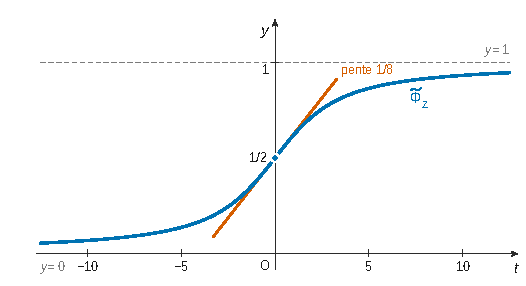
\includegraphics{figures/q2-2-2-graphe-phi-z.pdf}
\caption*{Figure 1 --- Graphe de Φ̃\_Z : valeur 1/2 et pente 1/8 en 0, asymptotes y
= 0 en −∞ et y = 1 en +∞}
\end{figure}

\hypertarget{uxe9tude-guxe9nuxe9rale-kge-2}{%
\subsection{\texorpdfstring{3. Étude générale (\(k\ge 2\))}{3. Étude générale (k\textbackslash ge 2)}}\label{uxe9tude-guxe9nuxe9rale-kge-2}}

\textbf{3.1.} Pour chaque \(i\), \(e^{x_it}=1+x_it+\frac{x_i^2t^2}{2}+o(t^2)\) (question 1, ou trivial si \(x_i=0\)). En sommant ces \(k\) développements, en nombre fini :
\equationajustee{G(t)=1+m_1t+\frac{m_2}{2}t^2+o(t^2),}
avec, par la formule de transfert,
\equationajustee{\begin{aligned}m_1&=\sum_ip_ix_i=\mathbb E(X),\\m_2&=\sum_ip_ix_i^2=\mathbb E(X^2).\end{aligned}}
Avec \(w=G(t)-1\), on a \(w^2=m_1^2t^2+o(t^2)\), d'où
\equationajustee{\ln G(t)=m_1t+\frac{m_2-m_1^2}{2}t^2+o(t^2).}
Comme \(m_2-m_1^2=V(X)\) (König-Huygens), on obtient en divisant par \(t\) :
\equationajustee{\boxed{\Phi_X(t)=\mathbb E(X)+\frac{V(X)}{2}\,t+o(t)\qquad(t\to 0).}}

\textbf{3.2.} Posons \(\widetilde\Phi_X(0)=\mathbb E(X)\) et \(\widetilde\Phi_X=\Phi_X\) sur \(\mathbb R^*\).

Par 3.1, \(\widetilde\Phi_X\) admet en \(0\) un développement limité d'ordre \(1\), donc elle est dérivable en \(0\).

Sur \(\mathbb R^*\), \(\widetilde\Phi_X=\frac{\ln G}{t}\) est de classe \(\mathcal C^\infty\), puisque \(G>0\) est \(\mathcal C^\infty\).

\textbf{\(\widetilde\Phi_X\) est dérivable sur \(\mathbb R\).}

\textbf{3.3.} \(\widetilde\Phi_X(0)=\lim_{t\to 0}\Phi_X(t)\) est le terme constant du développement de 3.1 :
\equationajustee{\boxed{\begin{aligned}\widetilde\Phi_X(0)&=\mathbb E(X)\\&=\sum_{i=1}^kp_ix_i.\end{aligned}}}

\textbf{3.4.} Le coefficient de \(t\) dans le développement limité d'ordre \(1\) est le nombre dérivé en \(0\) :
\equationajustee{\boxed{\widetilde\Phi_X'(0)=\frac{V(X)}{2},}}
la moitié de la variance de \(X\). On vérifie sur l'exemple de la question 2.2 : \(V(Z)=\frac14\) et \(\widetilde\Phi_Z'(0)=\frac18\).

\textbf{3.5.} Pour \(t>0\), on écrit \(G(t)=p_ke^{x_kt}(1+\varepsilon(t))\) avec \(\varepsilon(t)=\sum_{i<k}\frac{p_i}{p_k}e^{(x_i-x_k)t}\). On a \(\varepsilon(t)\to 0\) quand \(t\to+\infty\), car \(x_i<x_k\). Donc
\equationajustee{\Phi_X(t)=x_k+\frac{\ln p_k+\ln(1+\varepsilon(t))}{t}\xrightarrow[t\to+\infty]{}x_k.}
De même, pour \(t<0\), \(G(t)=p_1e^{x_1t}(1+\eta(t))\) avec \(\eta(t)=\sum_{i>1}\frac{p_i}{p_1}e^{(x_i-x_1)t}\), qui tend vers \(0\) quand \(t\to-\infty\). Donc \(\Phi_X(t)\to x_1\).
\equationajustee{\boxed{\begin{aligned}\lim_{+\infty}\widetilde\Phi_X&=x_k=\max_i x_i,\\\lim_{-\infty}\widetilde\Phi_X&=x_1=\min_i x_i.\end{aligned}}}

\textbf{3.6.} \textbf{Non.} Si \(\widetilde\Phi_X\) était impaire, elle vérifierait \(\widetilde\Phi_X(0)=0\) puisqu'elle est définie en \(0\), donc \(\mathbb E(X)=\sum_ip_ix_i=0\).

C'est une somme de termes positifs, avec \(p_i>0\) et \(x_i\ge 0\), donc tous les \(x_i\) seraient nuls. Cela contredit \(x_1<x_2\), puisque \(k\ge 2\).

Autre argument : l'imparité imposerait \(\lim_{-\infty}=-\lim_{+\infty}\), c'est-à-dire \(x_1=-x_k\), alors que \(0\le x_1<x_k\). \textbf{\(\widetilde\Phi_X\) n'est pas impaire.}

\textbf{4.} Par la formule de transfert, \(\mathbb E(e^{tX})=\sum_ip_ie^{tx_i}=G(t)>0\), d'où
\equationajustee{\boxed{\begin{aligned}{}&\forall t\in\mathbb R^*,\quad\Phi_X(t)=\frac1t\ln\mathbb E\left(e^{tX}\right),\\&\text{soit}\quad\mathbb E\left(e^{tX}\right)=e^{t\Phi_X(t)}.\end{aligned}}}

\textbf{5.} La variable \(X+Y\) est discrète finie, à valeurs dans \(\mathbb R_+\), donc \(\Phi_{X+Y}\) est définie. Soit \(t\in\mathbb R^*\).

Les variables \(e^{tX}\) et \(e^{tY}\) sont indépendantes, comme fonctions de variables indépendantes, et finies, donc d'espérance finie. D'où
\equationajustee{\mathbb E\left(e^{t(X+Y)}\right)=\mathbb E\left(e^{tX}\right)\mathbb E\left(e^{tY}\right).}
En prenant le logarithme (les trois espérances sont \(>0\)) puis en divisant par \(t\) :
\equationajustee{\boxed{\forall t\in\mathbb R^*,\quad\Phi_{X+Y}(t)=\Phi_X(t)+\Phi_Y(t).}}

\textbf{FIN}

\end{document}
